\documentclass[10pt]{beamer}

\usetheme[]{m}

\usepackage{booktabs}
\usepackage[scale=2]{ccicons}

\usepackage{pgfplots}
\usepgfplotslibrary{dateplot}

\title{Stochastic Optimization in Machine Learning}
\subtitle{Case Studies in Nonlinear Optimization}
\date{\today}
\author{F. Bauer \and S. Chambon \and R. Halbig \and S. Heidekrüger \and J. Heuke}
\institute{Technische Universität München}
% \titlegraphic{\hfill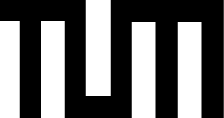
\includegraphics[height=1.5cm]{logo/logo}}

\begin{document}

\maketitle

\begin{frame}
  \frametitle{Awesome Motivational Title}
  Awesome Motivational Slide.\\
  \emph{Yeah!}
\end{frame}

\begin{frame}
  \frametitle{Table of Contents}
  \setbeamertemplate{section in toc}[sections numbered]
  \tableofcontents[hideallsubsections]
\end{frame}

\section{Introduction}

  \begin{frame}
    \frametitle{Introduction}
    What are we doing?
    Why?
  \end{frame}

\section{A Stochastic Quasi Newton Method}

  \begin{frame}
    \frametitle{Stochastic Quasi Newton}
      What is it?\cite{SQN}
      Why?
      Main ideas, high-level pseudo code overview?
      short bfgs repitition?
      Extreme Cases (L-BFGS, SGD)
  \end{frame}

  \begin{frame}
    \frametitle{HIGGS-Dataset}
    Explain the Dataset quickly.
    Why is this good for SQN testing?
    Why is it challenging? (file size etc)
  \end{frame}

  \begin{frame}
    \frametitle{Behavior}
      Pretty picures about the behaviour of SQN on HIGGS
      and comparison with traditional SGD
  \end{frame}

 \section{Proximal Splitting Method}

   \plain{Outline of Section by Jacob and Fin}
   \begin{frame}\frametitle{First Prox Slide}
       \begin{itemize}
            \item hallo
            \item \alert{du muschi}
            \item \cite{becker2012quasi}
          \end{itemize}   
   
   \end{frame}

\section{Logistic Regression: An Example}
  \begin{frame}\frametitle{Task}
    Explain what we want to do, and explain the dataset,
    and why using both SQN and Prox makes sense   
  \end{frame}

  \begin{frame}\frametitle{Results}
    Nice table with SQN, SGD (no reg, L2), (Lasso,) Prox (L1) showing
    Obj. value in found optimum, CPU time, Iterations, F1 score of prediction model

    Use different reg. parameters??
    Stop after fixed time? after fixed iters? after insign. improvements  
  \end{frame}

\section{Conclusion}

  \begin{frame}{Summary}
    \begin{center}\ccbysa\end{center}
  \end{frame}

  \plain{Questions?}

  \begin{frame}[allowframebreaks]\frametitle{Main References}

    \bibliography{refs}
    \bibliographystyle{abbrv}

  \end{frame}

\end{document}
